\documentclass[11pt,a4paper]{article}
\usepackage[utf8]{inputenc}
\usepackage[ngerman]{babel}
\usepackage{csquotes}
\usepackage{graphicx}
\usepackage{geometry}
\usepackage{hyperref}
\usepackage{subfiles}
\usepackage{amssymb} 
\usepackage{amsmath}
\usepackage{tabularx}
\usepackage{colortbl}
\usepackage{color}
\usepackage[rgb]{xcolor}
\usepackage{afterpage}
\usepackage[style=apa, backend=biber]{biblatex}
% \usepackage{indentfirst} 
% \usepackage[
%     colorlinks=true, 
%     linkcolor=blue,
%     urlcolor=blue,
%     citecolor=blue,
%     anchorcolor=blue
% ]{hyperref}

\addbibresource{references.bib}
\geometry{a4paper, total={170mm,257mm}, left=20mm, top=20mm}
\definecolor{ba-gray}{rgb}{0.9,0.9,0.9}

\newcommand\blankpage{%
    \null
    \thispagestyle{empty}%
    \addtocounter{page}{-1}%
    \newpage}

\newcommand\redpage{%
    \newpage
    \pagecolor{red}
    \blankpage
    \afterpage{\nopagecolor}}



\title{
    {\LARGE Bachelorarbeit}\\[2em]
    {\textbf{Integration einer Sprachsteuerungsfunktion {\break} in Mobile Apps}}
}
\author{Rubén Nuñez}
\date{Herbstsemester 2023}

\begin{document}

\maketitle
\thispagestyle{empty} %Keine Seitennummerierung auf der start Seite
\newpage

\section*{Bachelorarbeit an der Hochschule Luzern -- Informatik}
\subfile{affidavit.tex}
\newpage


\section*{Abstract}
Das Problem dieser Arbeit ist im wesentlichen die Erkennung von Triggerwörtern innerhalb
des Kontext einer App. Grundsätzlich ist es unüblich, dass mobile Apps eine
integrierte Sprachsteuerungsfunktion anbieten.

\newpage
\tableofcontents

\newpage
\section{Problem, Fragestellung, Vision}
Das Kernproblem dieser Bachelorarbeit ist die Erkennung von Triggerwörtern innerhalb eines 
App-Kontexts. Obwohl Sprachsteuerungstechnologien ein erhebliches Potenzial aufweisen und 
Assistenten wie Siri oder Alexa weit verbreitet sind, bieten mobile Apps selten eine integrierte 
Spracherkennung. Dies führt zu einer Lücke, da solche Assistenten nicht spezifisch für App-Kontexte 
optimiert sind. Diese Arbeit verfolgt das Ziel, diese Lücke zu schliessen und eine integrierte 
Spracherkennungsfunktion zu entwickeln, die Triggerwörter in einer App effektiv erkennt.

\subsection{Fragestellung}
Die Fragestellung dieser Arbeit lautet: \textit{Wie kann eine integrierte Sprachsteuerung für eine
Mobile Apps entwickelt werden, die speziell das Erkennen von Triggerwörtern ermöglicht, indem 
Methoden des Machine Learnings genutzt werden?}.

\subsection*{Ausgangslage und Problemstellung}
Sprachsteuerungstechnologien haben ein grosses Potenzial und werden bisher vor allem als
Sprachsteuerungsassistenten genutzt. Während es etablierte Sprachassistenten wie Siri gibt,
fehlt es an Lösungen für eine integrierte Sprachsteuerung in Mobile Apps, insbesondere in
Bezug auf das Erkennen von Triggerwörtern.

\subsection*{Ziel der Arbeit und erwartete Resultate}
Ziel der Arbeit ist es zum einen, eine Grundlage zu schaffen, um ein Triggerwort oder eine
Sequenz von Triggerwörtern in der akustischen Sprache erkennen zu können. Dabei werden
Methoden und Werkzeuge aus dem Bereich des Machine Learnings verwendet. Zum anderen soll
diese Erkenntnis in eine mobile Plattform wie iOS oder Android integriert werden. Für den
Rahmen dieser Arbeit genügt die Integration in eine der genannten Plattformen. Weiterhin
werden das Thema Datenschutz und die ethischen Aspekte berücksichtigt.

\subsection*{Gewünschte Methoden, Vorgehen}
Das Projekt kann beispielsweise in drei Phasen durchgeführt werden: Technische Abklärungen,
Datensammlung und Modelltraining, sowie die Erarbeitung eines Prototypen. Agile
Vorgehensweisen sind wünschenswert.

\subsection*{Kreativität, Methoden, Innovation}
Bisher sind Sprachsteuerungsfunktionen fast ausschliesslich grossen Akteuren wie Siri
vorbehalten. Der innovative Ansatz dieser Arbeit zielt darauf ab, einen Anreiz zu setzen,
um diese Funktionen auch in herkömmlichen Apps einzusetzen. Die handfreie Bedienung durch
Sprachsteuerung hat das Potenzial, das Benutzererlebnis erheblich zu verbessern.



\newpage
\section{Stand der Forschung}
Um diese Arbeit fundiert anzugehen, ist ein Verständnis der Grundlagen in den Bereichen 
Audioverarbeitung und Machine Learning essenziell. Daher wird in diesem Kapitel ein Überblick 
über die wichtigsten Themen gegeben. Zudem wird das Kapitel sich mit der Implementation von 
Sprachsteuerungstechnologien befassen. Darunter fallen die Sprachassistenten wie Siri, Alexa oder 
Google Assistant. Was natürlich auch nicht fehlen darf, ist eine kleine Einleitung in die 
Fourier-Transformation. Die Fourier-Transformation ist ein wichtiges Konzept in der 
Signalverarbeitung und wird in dieser Arbeit verwendet.



\subsection{Audio}
In der digitalen Welt repräsentiert Audio Schallwellen, die durch eine Reihe von numerischen Werten 
dargestellt werden \cite[p.9]{somberg2019audioapi}. beschreibt Audio als: \glqq Fundamentally, 
audio can be modeled as waves in an elastic medium. In our normal everyday experience, the elastic 
medium is air, and the waves are air pressure waves.\grqq \ Audiosignale werden durch die Funktion
\(A(t)\) repräsentiert, wobei \(t\) die Zeit und \(A(t)\) die Amplitude zum
Zeitpunkt \(t\) angibt. Die Amplitude ist die Stärke des Signals und die Zeit repräsentiert die
Position des Signals in der Zeit. Diese Betrachtung ist vor allem in der Elektrotechnik
von Bedeutung, da die Amplitude als Spannung angesehen werden kann. Grundsätzlich ist Audio ein
kontinuierliches Signal. In der digitalen Welt können wir jedoch nur diskrete Werte darstellen.
Daher wird das kontinuierliche Signal in diskrete Werte umgewandelt. Dieser Vorgang wird als
\textit{Sampling} bezeichnet (\cite[Chapter~3.1]{tarr2018hackaudio}). 


\subsubsection{Sampling}
Ein früher Ansatz zur digitalen Darstellung von analogen Signalen war die Pulse-Code-Modulation
(PCM). Dieses Verfahren wurde bereits in den 1930er Jahren von Alec H. Reeves entwickelt,
parallel zum Aufkommen der digitalen Telekommunikation (\cite[p.~57]{deloraine1965pcm}).
Im Grundsatz wird es heute noch in modernen Computersystemen nach dem gleichen Verfahren angewendet.

\noindent
\newline
Es folgt eine formelle Definition von Sampling. Ein kontinuierliches Signal \(A(t)\)
wird in bestimmten Zeitintervallen \(T_s\) gesampelt. Diese Zeitintervalle werden auch als
Sampling-Periode bezeichnet. Die Sampling-Rate \(F_s = \displaystyle\frac{1}{T_s}\) gibt die Anzahl
der Samples pro Sekunde an. Angenommen wir haben ein Signal mit einer Sampling-Periode
von \(T_s = 0.001\). Um nun die Sampling-Rate zu berechnen, müssen wir den Kehrwert der
Sampling-Periode berechnen. \(F_s = \displaystyle\frac{1}{0.001} = 1000\). Somit erhalten wir eine
Sampling-Rate von \(1000\) Samples pro Sekunde. Nun typische Sampling-Raten sind \(44100\) Hz
oder \(48000\) Hz. Bei Sampling-Raten wird die Einheit \textit{Hertz} verwendet. Ein Hertz entspricht
einer Frequenz von einem Sample pro Sekunde. Ein weiter wichtiger Begriff ist die
\textit{Nyquist-Frequenz}. Die Nyquist-Frequenz \(F_n\) ist die Hälfte der Sampling-Rate.
Also \(F_n = \displaystyle\frac{F_s}{2}\). Die Idee hinter der Nyquist-Frequenz ist, dass die
Sampling-Rate mindestens doppelt so hoch sein muss wie die höchste Frequenz des Signals. Wenn diese
Eigenschaft erfüllt ist, kann das Signal ohne Informationsverlust rekonstruiert werden 
(\cite[Chapter~3.1]{tarr2018hackaudio}). Mehr dazu folgt im Unterkapitel 
\textit{Fourier-Transformation}.


\noindent
\newline
Weiter ist es wichtig zu verstehen, dass ein Sample ein diskreter Wert ist. Und dieser wird in
digitalen Systemen durch eine bestimmte Anzahl von Bits dargestellt. Die Anzahl der Bits wird
als \textit{Bit-Depth} bezeichnet. Die Bit-Depth bestimmt die Auflösung des Signals. Typische
Bit-Depth Werte sind \(16\) oder \(24\) Bit (\cite[p.10]{somberg2019audioapi}). 

\subsubsection{Frames, Channels, Buffers}
Ebendfalls wichtig ist das Verständnis von Frames, Channels und Buffers. Da diese Arbeit sich mit
Audio-Systemen beschäftigt, ist es wichtig, die Begriffe \textit{Frame}, \textit{Channel} und
\textit{Buffer} zu verstehen. Fangen wir mit dem Begriff \textit{Channel} an. Ein Channel kann als
ein einzelnes Audio-Signal angesehen werden. Ein Mono-Signal hat genau nur einen Channel. Ein
Stereo-Signal hat zwei Channels. Ein Surround-Signal hat mehr als zwei Channels. usw.
Nun zum Begriff \textit{Frame}. Ein Frame entspricht einem Sample pro Channel. Weiter sind Frames 
in Buffers organisiert. Ein Buffer ist eine Sammlung von Frames. Typischerweise werden Buffers in 
Grössen von \(64\), \(128\), \(256\), \(512\) oder \(1024\) Frames organisiert. Die Abbildung 
\ref{fig:frames_channels_buffers} zeigt die Beziehung zwischen Frames, Channels und Buffers. 
Die Abbildung wurde basierend auf (\cite[p.10]{somberg2019audioapi}) erstellt und verdeutlicht die
Beziehung zwischen Frames, Channels und Buffers.

\begin{figure}[h]
    \centering
    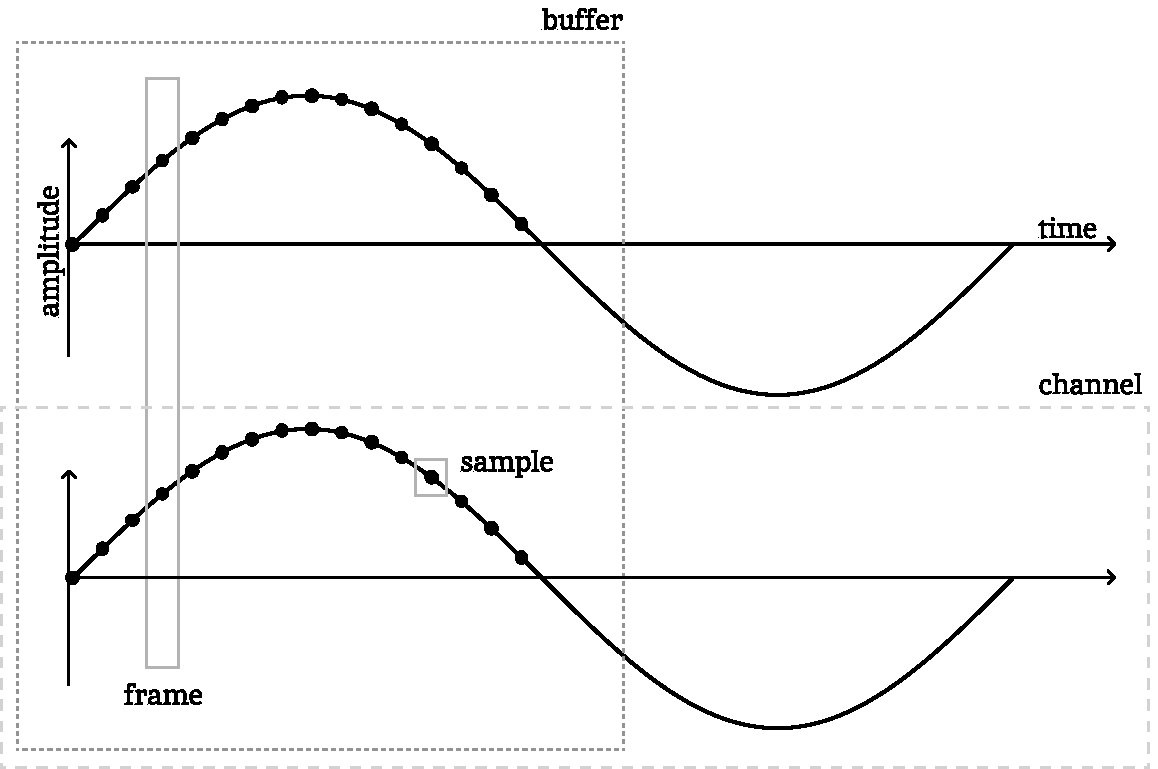
\includegraphics[width=0.7\linewidth]{img/audio-nutshell.pdf}
    \caption{Frames, Channels und Buffers}
    \label{fig:frames_channels_buffers}
\end{figure}


\subsubsection{Buffers im Detail}
Ein Buffer im Kontext von Audio ist eine aufeinanderfolgende Sammlung von Frames. Die bereits
angesprochene Grösse eines Buffers bestimmt im wesentlichen die Latenzzeit des Systems. Kleine
Buffer-Grössen haben eine geringe Latenzzeit, während grosse Buffer-Grössen eine hohe Latenzzeit 
haben (\cite[p.10]{somberg2019audioapi}). Der Trade-Off ist dass kleine Buffer-Grössen 
zu einer höheren CPU-Auslastung führen, während bei grossen Buffer-Grössen das nicht der Fall ist.
Das liegt daran, dass bei kleinen Buffer-Grössen die CPU häufiger aufgerufen wird, um die Buffers
zu verarbeiten. 

\noindent
\newline
Nun betrachten wir die Anordnung der Frames in einem Buffer, wie in den folgenden Abbildungen 
dargestellt. Es gibt zwei Möglichkeiten, wie die Frames in einem Buffer angeordnet werden 
können: \textit{Interleaved} und \textit{Non-Interleaved}. Bei der \textit{Interleaved}-Anordnung 
werden die Frames der einzelnen Channels nacheinander in sequentieller Reihenfolge in den Buffer 
geschrieben. Im Gegensatz dazu werden bei der \textit{Non-Interleaved}-Variante die Frames 
eines Channels nacheinander in den Buffer geschrieben, bevor die Frames des nächsten Channels 
hinzugefügt werden. Dieser Vorgang wird für jeden Channel wiederholt. Die Abbildung 
\ref{fig:frames_buffers} zeigt die Unterschiede zwischen den beiden Anordnungen. Die Abbildung 
wurde basierend auf (\cite[p.11]{somberg2019audioapi}) erstellt.


\begin{figure}[h]
    \centering
    \begin{tabularx}{\textwidth}{|X|X|X|X|X|X|X|X|}
    \hline
    L & R & L & R & L & R & L & R \\
    \hline
    L & L & L & L & R & R & R & R \\
    \hline
    \end{tabularx}

    
    \caption{Frames in Interleaved und Non-interleaved Buffers}
    \label{fig:frames_buffers}
\end{figure}

\noindent
\newline
Mit diesem Wissen können wir nun die Unterschiede zwischen den beiden Anordnungen. Für die 
Anwendung ist es wichtig zu verstehen, mit welcher Anordnung die verwendete API arbeitet.


\subsection{Fourier-Transformation}
Die Fourier-Transformation ist ein zentrales Werkzeug der Fourier-Analyse, einem Teilgebiet der 
Mathematik, das sich mit der Zerlegung von Funktionen in Frequenzkomponenten beschäftigt. 
Im Kern handelt es sich bei der Fourier-Analyse um die Approximation einer Funktion durch 
Überlagerung von Schwingungen mit unterschiedlichen Frequenzen. Dieses Konzept wird auch von 
Prof. Dr. Weitz in seinem Youtube Video erläutert (\cite[2:20]{weitz2023fourier}). 
Mathematisch ausgedrückt kann die kontinuierliche Fourier-Transformation eines Signals \( f(t) \) 
wie folgt definiert werden:

\begin{equation*}
F(\omega) = \int_{-\infty}^{\infty} f(t) e^{-i \omega t} \, dt
\label{eq:fourier_transform}
\end{equation*}

\noindent
\newline
\(F(\omega)\) ist die kontinuierliche Fourier-Transformation von \(f(t)\) 
(\cite[49:27]{weitz2023fourier}). Als kleines Rechenbeispiel betrachten wir die kontinuierliche
Fourier-Transformation der einfachen periodischen Funktion \(f(t) = sin(t) + \frac{1}{2}sin(2t)\). 

\noindent
\newline
Um die Fourier-Transformation für \( f(t) = \sin(t) + \frac{1}{2}\sin(2t) \) zu berechnen, 
gehen wir schrittweise vor:

\noindent
\newline
\textbf{1. Zerlegung des Signals:}  
Zunächst zerlegen wir \( f(t) \) in seine beiden Komponenten: \( \sin(t) \) und 
\( \frac{1}{2}\sin(2t) \). Die Fourier-Transformation wird für jede dieser Komponenten separat 
berechnet und die Ergebnisse werden dann zusammengefasst.

\noindent
\newline
\textbf{2. Fourier-Transformation von \( \sin(t) \):}  
Die Fourier-Transformation von \( \sin(t) \) ergibt zwei Delta-Funktionen in der Frequenzdomäne, 
jeweils bei \( \omega = 1 \) und \( \omega = -1 \). Die Fourier-Transformation für \( \sin(t) \) 
lautet:

\begin{equation*}
\mathcal{F}\{\sin(t)\} = i \left( \delta(\omega + 1) - \delta(\omega - 1) \right)
\end{equation*}

\noindent
\newline
\textbf{3. Fourier-Transformation von \( \frac{1}{2}\sin(2t) \):}  
Ähnlich wie im vorherigen Schritt, ergibt die Fourier-Transformation von \( \frac{1}{2}\sin(2t) \) 
zwei Delta-Funktionen bei \( \omega = 2 \) und \( \omega = -2 \). Die Fourier-Transformation für 
\( \frac{1}{2}\sin(2t) \) lautet:

\begin{equation*}
\mathcal{F}\{\frac{1}{2}\sin(2t)\} = \frac{i}{2} \left( \delta(\omega + 2) - 
\delta(\omega - 2) \right)
\end{equation*}

\noindent
\newline
Das Zusammenfassen der beiden Ergebnisse ergibt die endgültige Fourier-Transformierte für 
\( f(t) = \sin(t) + \frac{1}{2}\sin(2t) \):

\begin{equation*}
F(\omega) = \frac{i}{2} \left( \delta(\omega + 1) - \delta(\omega - 1) \right) + 
\frac{i}{4} \left( \delta(\omega + 2) - \delta(\omega - 2) \right)
\end{equation*}


\noindent
\newline
Die diskrete Fourier-Transformation (DFT) ist eine diskrete Version der Fourier-Transformation.
Welche die Fourier-Transformation auf diskrete Signale anwendet. Die DFT ist näher an der
Anwendung, da Signale in digitalen Systemen diskret sind.








\newpage
\section{Ideen und Konzepte}
Das Problem dieser Arbeit ist im wesentlichen die Erkennung von Triggerwörtern innerhalb
des Kontext einer App. Grundsätzlich ist es unüblich, dass mobile Apps eine
integrierte Sprachsteuerungsfunktion anbieten.


\newpage
\section{Methoden}
Das Problem dieser Arbeit ist im wesentlichen die Erkennung von Triggerwörtern innerhalb
des Kontext einer App. Grundsätzlich ist es unüblich, dass mobile Apps eine
integrierte Sprachsteuerungsfunktion anbieten.


\newpage
\section{Realisierung}
Das Problem dieser Arbeit ist im wesentlichen die Erkennung von Triggerwörtern innerhalb
des Kontext einer App. Grundsätzlich ist es unüblich, dass mobile Apps eine
integrierte Sprachsteuerungsfunktion anbieten.


\newpage
\section{Evaluation und Validation}
Das Problem dieser Arbeit ist im wesentlichen die Erkennung von Triggerwörtern innerhalb
des Kontext einer App. Grundsätzlich ist es unüblich, dass mobile Apps eine
integrierte Sprachsteuerungsfunktion anbieten.

\newpage
\section{Ausblick}
Das Problem dieser Arbeit ist im wesentlichen die Erkennung von Triggerwörtern innerhalb
des Kontext einer App. Grundsätzlich ist es unüblich, dass mobile Apps eine
integrierte Sprachsteuerungsfunktion anbieten.


\newpage
\section{Anhang}
\subfile{projectmanagement.tex}
\newpage

% Verzeichnisse
\addcontentsline{toc}{section}{Abbildungsverzeichnis}
\listoffigures
\addcontentsline{toc}{section}{Tabellenverzeichnis}
\listoftables
\printbibliography[title=Literaturverzeichnis, heading=bibintoc]



%       %%%%%   %    %   %%%
%       %       % %  %   %   %
%       %%%%    %  % %   %    %
%       %       %   %%   %   %
%       %%%%%   %    %   %%%


\newpage
\pagecolor{ba-gray}
\afterpage{\nopagecolor}
\blankpage

\newpage
\section*{Aufgabenstellung}
Integration von Sprachsteuerungstechnologien in Mobile Apps, insbesondere zur Erkennung
von Triggerwörtern.

\section*{Projektteam}
\begin{itemize}
    \item Student:in: Rubén Nuñez
    \item Betreuer:in: Herzog
    \item Firma: Bitforge AG
\end{itemize}

\section*{Auftraggeber}
\begin{itemize}
    \item Firma: Bitforge AG
    \item Ansprechperson: Stefan Reinhard
    \item Funktion: Head of Mobile
    \item Adresse: Zeughausstrasse 39, 8004 Zürich
    \item Telefon: +41 55 211 02 41
    \item E-Mail: stefan.reinhard@bitforge.ch
    \item Website: www.bitforge.ch
\end{itemize}



\section*{Sonstige Bemerkungen}
Grundkenntnisse in Machine Learning, speziell im Bereich der Spracherkennung, sowie
Erfahrung mit entsprechenden APIs sind erforderlich.






\end{document}
